\documentclass{report}
\usepackage{amsmath}
\usepackage{ngerman}
\usepackage[hidelinks]{hyperref}
\usepackage[numbered]{bookmark}
\usepackage{pgfplots}
\usepgfplotslibrary{fillbetween}
\pgfplotsset{compat=1.18}
\tracinglostchars=2

\title{\textbf{Mathe-Abitur}}
\author{Tim Teichmann}
\date{\today}

\begin{document}
\maketitle
\tableofcontents

\chapter{Funktionsscharen}

\section{Definition}
\begin{flushleft}
    Eine Funktionsschar ist eine Funktion, die auch von anderen Parametern als \(x\) abhängt.
    \begin{align}
        f_k(x)=kx^2
    \end{align}
    Das ist beispielsweise eine quadratische Funktionsschar, die von den Parametern \(x\) und \(k\) abhängt.
\end{flushleft}

\begin{center}
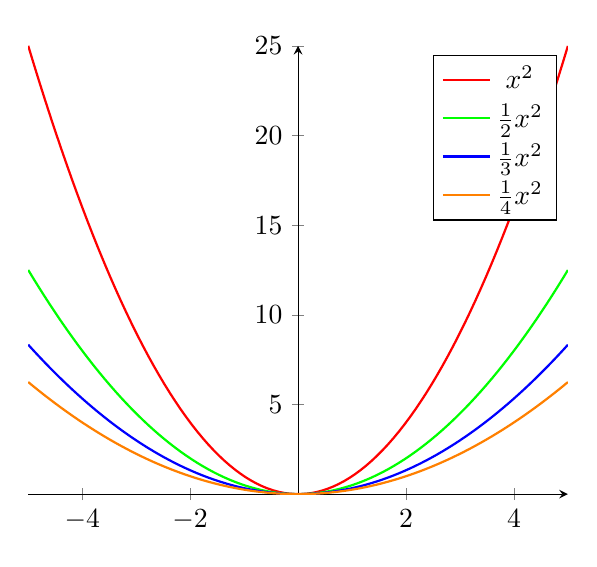
\begin{tikzpicture}
\begin{axis}[
    axis lines=middle,
    samples=100,
    domain=-5:5,
    every axis plot/.append style={thick},
]
\addplot[
    color=red,
]
{x^2};
\addlegendentry{\(x^2\)}

\addplot[
    color=green,
]
{0.5*x^2};
\addlegendentry{\(\frac{1}{2}x^2\)}

\addplot[
    color=blue,
]
{0.3333*x^2};
\addlegendentry{\(\frac{1}{3}x^2\)}

\addplot[
    color=orange,
]
{0.25*x^2};
\addlegendentry{\(\frac{1}{4}x^2\)}

\end{axis}
\end{tikzpicture}
\end{center}

\begin{flushleft}
    Anhand von diesem Beispiel kann man relativ einfach erkennen, dass Funktionen durch Parameter verschiedene Eigenschaften aufweisen können.
\end{flushleft}

\chapter{Trassierungsaufgaben}

\section{Definition}

\begin{flushleft}
    Das Ziel von Trassierungsaufgaben ist es anhand von bestimmten Angaben eine Funktion aufzustellen.
    Deshalb ist das Verstehen der Aufgabenstellung der schwierigste Teil der Aufgabe.
\end{flushleft}

\section{Beispiel}

\begin{flushleft}
    Das ist eine mögliche Aufgabenstellung: \\
    \textit{Eine quadratische Funktion hat im Punkt $P(0|0)$ eine Nullstelle und im Punkt $Q(2|5)$ ein Maximum. Stelle die Funktionsgleichung auf!} \\
    \begin{enumerate}
        \item {
                Die ersten drei Wörter des Satzes: \textbf{\textit{Eine quadratische Funktion}} sagen uns um welchen Typ Funktion es sich handelt.
                Es ist eine quadratische Funktion. Die allgemeine quadratische Funktion sieht so aus:
                \begin{align}
                    f(x)=ax^2+bx+c
                \end{align}
                Unsere Funktion $f$ hat also drei unbekannte, $a$, $b$ und $c$.
            }
        \item {
                Außerdem ist für uns wichtig, dass die Funktion \textbf{\textit{im Punkt $P(0|0)$ eine Nullstelle}} hat.
                Das bedeutet, dass $f(0)=0$ sein muss.
                Unsere erste Bedingung ist also:
                \begin{align}
                    f(0)=0
                \end{align}
            }
        \item {
                Als letztes hat unsere Funktion \textbf{\textit{im Punkt $Q(2|5)$ ein Maximum}}. \\
                Um die Extrempunkte von einer Funktion (hier: $g$) zu finden, muss man die erste Ableitung dieser Funktion gleich $0$ setzen.
                \begin{align}
                    g'(x)=0
                \end{align}
                Im Idealfall bekommt man eine oder mehr Lösungen heraus, wir nennen die Lösung $x_1$.
                Um herauszufinden um welche Art von Extrempunkt es sich handelt setzen wir $x_1$ in die zweite Ableitung von $g$ ein.
                \begin{align}            
                    g''(x) =
                    \begin{cases}
                        \text{Maximum}, &\text{wenn } x < 0 \\
                        \text{Minimum}, &\text{wenn } x > 0
                    \end{cases}
                \end{align}
                Jetzt können wir drei weitere Bedingungen für unsere Aufgabe aufstellen.
                Unsere Funktion soll ein Maximum in $Q(2|5)$ haben, deshalb müssen diese Bedingungen erfüllt sein:
                \begin{align}
                    f(2)=5 \\
                    f'(2)=0 \\
                    f''(2) < 0
                \end{align}
            }
        \item {
                Jetzt müssen wir aus unseren vier Bedingungen eine Funktion bilden, dafür bilden wir erstmal die ersten beiden Ableitungen.
                \begin{align}
                    f(x)&=ax^2+bx+c \\
                    f'(x)&=2ax+b \\
                    f''(x)&=2a \\
                    f(0)&=0 \\
                    f(2)&=5 \\
                    f'(2)&=0 \\
                    f''(2) & < 0
                \end{align}
                Nun müssen wir einsetzen, Ungleichungen ($f''(2) < 0$) dürfen nicht eingesetzt werden.
                \begin{align}
                    0^2a+0b+c &=0 \\
                    c &=0 \\
                    a*2^2+2b+c &= 5 \\
                    4a+2b+c &= 5 \\
                    4a+2b &= 5 \\
                    2a*2+b &=0 \\
                    4a+b &= 0
                \end{align}
                Eine von den drei unbekannten ist gelöst ($c=0$).
                Jetzt muss $4a+2b=5$ in $4a+b=0$ eingesetzt werden.
                \begin{align}
                    4a+2b &=5 \\
                    4a+b &= 0 \\
                    4a+2b-(4a+b) &= 5 \\
                    b &= 5 \\
                    4a+5 &= 0 \\
                    a &= \frac{-5}{4}
                \end{align}
                Alle unbekannten Variablen sind gelöst, $a=\frac{-5}{4}$, $b=5$, $c=0$.
                Also ist das unsere Funktion:
                \begin{align}
                    f(x)=\frac{-5}{4}x^2+5x
                \end{align}
            }
    \end{enumerate}
\end{flushleft}

\begin{center}
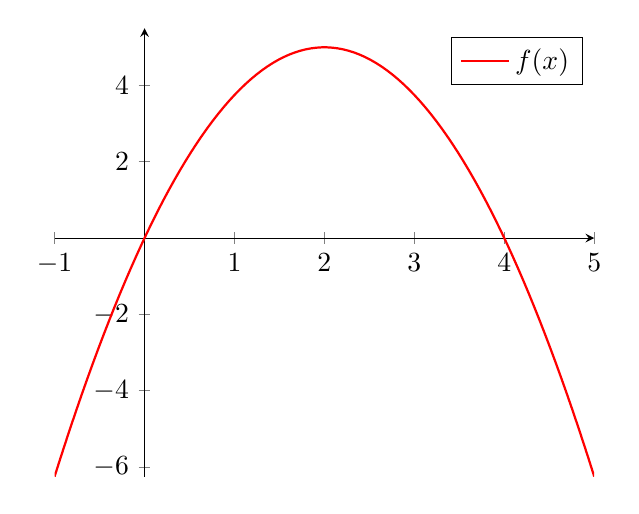
\begin{tikzpicture}   
\begin{axis}[
    axis lines=middle,
    samples=100,
    domain=-1:5,
    ymax=5.5,
    every axis plot/.append style={thick},
]
\addplot[
    color=red,
]
{(-5/4)*((\x)*(\x))+(5)*(\x)};
\addlegendentry{$f(x)$}

\end{axis}
\end{tikzpicture}
\end{center}

\chapter{Extremwertaufgaben}

\section{Definition}
\begin{flushleft}   
    Bei Extemwertaufgaben geht es darum die maximal/minimal möglichen Flächeninhalte herauszufinden.
    Dabei kann es oft auch um das maximale/minimale Volumen eines Körpers gehen.
    Jedoch maximiert/minimiert sich das Volumen eines Körpers wenn der Flächeninhalt des Mantels maximal/minimal wird.
    Die Aufgabenstellungen zu diesem Aufgabentyp sind meistens sehr spezifisch und brauchen eine Skizze.
\end{flushleft}

\section{Beispiel}
\begin{flushleft}
    In diesem Beispiel soll der maximale Flächeninhalt eines Dreiecks gefunden werden.
    Das Dreieck ist unterhalb der Funktion $f$.
    Die drei Ecken des Dreiecks sind die Punkte $P(u|v)$, $Q(0|0)$ und $R(u|0)$.
    \begin{align}
        f(x)=x^3-6x^2+9x
    \end{align}
\end{flushleft}

\begin{center}
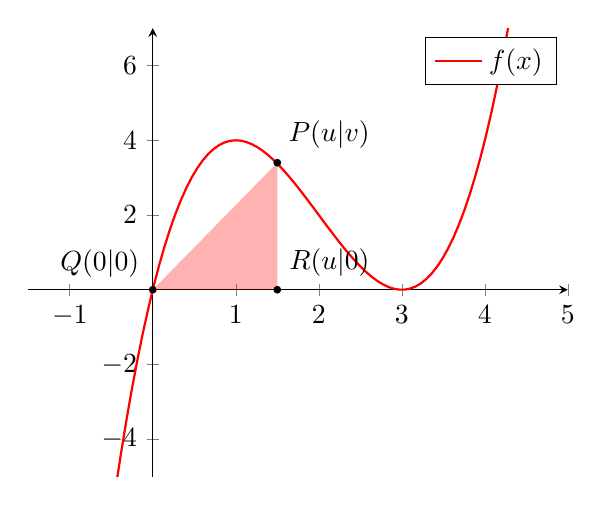
\begin{tikzpicture}   
\begin{axis}[
    axis lines=middle,
    samples=100,
    domain=-1.5:5,
    ymax=7,
    ymin=-5,
    every axis plot/.append style={thick},
]
\addplot[
    color=red,
    name path=A
]
{((\x)*(\x)*(\x))-(6*(\x)*(\x))+(9*(\x))};
\addlegendentry{$f(x)$}

\addplot[draw=none,name path=B] {(3.4/1.5)*(\x)};
\addplot[draw=none,name path=C] {0};
\addplot[red,opacity=0.3] fill between[of=B and C,soft clip={domain=0:1.5}];

\node[label={150:{$Q(0|0)$}},circle,fill,inner sep=1pt] at (axis cs:0,0) {};
\node[label={70:{$P(u|v)$}},circle,fill,inner sep=1pt] at (axis cs:1.5,3.4) {};
\node[label={60:{$R(u|0)$}},circle,fill,inner sep=1pt] at (axis cs:1.5,0) {};

\end{axis}
\end{tikzpicture}
\end{center}

\begin{flushleft}
    Um die Fläche $A$ eines Dreiecks auszurechnen nutzt man diese Formel, $g$ steht für die Grundseite und $h$ für die Höhe:
    \begin{align}
        A=\frac{gh}{2}
    \end{align}
    Mit $g$ und $h$ sieht der Plot so aus:
\end{flushleft}

\begin{center}
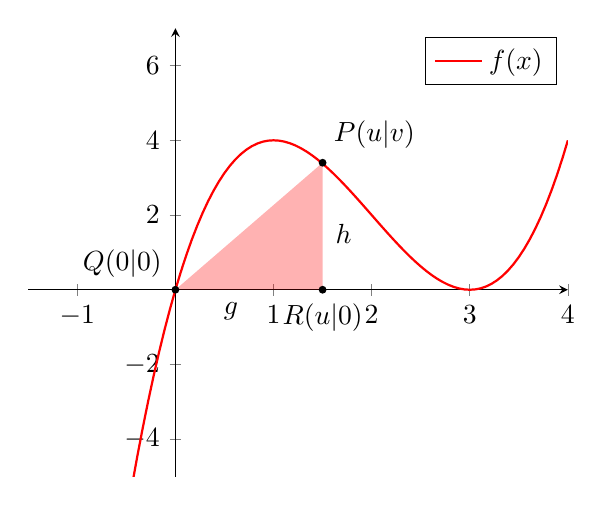
\begin{tikzpicture}   
\begin{axis}[
    axis lines=middle,
    samples=100,
    domain=-1.5:4,
    ymax=7,
    ymin=-5,
    every axis plot/.append style={thick},
]
\addplot[
    color=red,
    name path=A
]
{((\x)*(\x)*(\x))-(6*(\x)*(\x))+(9*(\x))};
\addlegendentry{$f(x)$}

\addplot[draw=none,name path=B] {(3.4/1.5)*(\x)};
\addplot[draw=none,name path=C] {0};
\addplot[red,opacity=0.3] fill between[of=B and C,soft clip={domain=0:1.5}];

\node[label={150:{$Q(0|0)$}},circle,fill,inner sep=1pt] at (axis cs:0,0) {};
\node[label={70:{$P(u|v)$}},circle,fill,inner sep=1pt] at (axis cs:1.5,3.4) {};
\node[label={270:{$R(u|0)$}},circle,fill,inner sep=1pt] at (axis cs:1.5,0) {};

\node[label={0:{$h$}},draw=none,inner sep=1pt] at (axis cs:1.5,1.5) {};
\node[label={250:{$g$}},draw=none,inner sep=1pt] at (axis cs:0.75,0) {};

\end{axis}
\end{tikzpicture}
\end{center}

\begin{flushleft}
    In unserem Beispiel ist $g=u$ und $h=v$, dazu ist $v=f(u)$.
    Wenn wir diese Werte in $A$ einsetzen bildet sich diese Funktion:
    \begin{align}
        A(u) &=\frac{u*f(u)}{2} \\
        A(u) &=\frac{u \left(u^3-6u^2+9u\right)}{2} \\
        A(u) &=\frac{u^4-6u^3+9u^2}{2} \\
        A(u) &=\frac{u^4}{2}-3u^3+\frac{9}{2}u^3
    \end{align}
    Unsere neue Funktion $A(u)$ kann jetzt den Flächeninhalt für jeden Wert von $u$ berechnen.
    Wir brauchen den maximalen Flächeninhalt, also soll die Funktion für den Flächeninhalt ($A(u)$) maximal werden.
    Um ein maximum zu berechnen bilden wir die ersten zwei Ableitungen unserer Funktion.
    \begin{align}
        A(u) &=\frac{u^4}{2}-3u^3+\frac{9}{2}u^3 \\
        A'(u) &= 2u^3-9u^2+9u \\
        A''(u) &= 6u^2-18u+9
    \end{align}
    Jetzt finden wir die Nullstelle der ersten Ableitung.
    \begin{align}
        A'(u) &=0 \\
        \iff u_1=0, u_2 &=\frac{3}{2}, u_3=3
    \end{align}
    Danach prüfen wir, in welcher Stelle ein Maximum liegt.
    \begin{align}
        A''\left(0\right) = 9 & > 0 \Longrightarrow \text{Minimum} \\
        A''\left(\frac{3}{2}\right) = \frac{-9}{2} & < 0 \Longrightarrow \text{Maximum} \\
        A''\left(3\right) = 9 & > 0 \Longrightarrow \text{Minimum} \\
        A\left(\frac{3}{2}\right) &= \frac{81}{32} \\
        v=f\left(\frac{3}{2}\right) &= \frac{27}{8}
    \end{align}
    Der größte Flächeninhalt ist $\frac{81}{32}$, um diesen zu erreichen muss $u=\frac{3}{2}$ und $v=\frac{27}{8}$ sein.
\end{flushleft}

\begin{center}
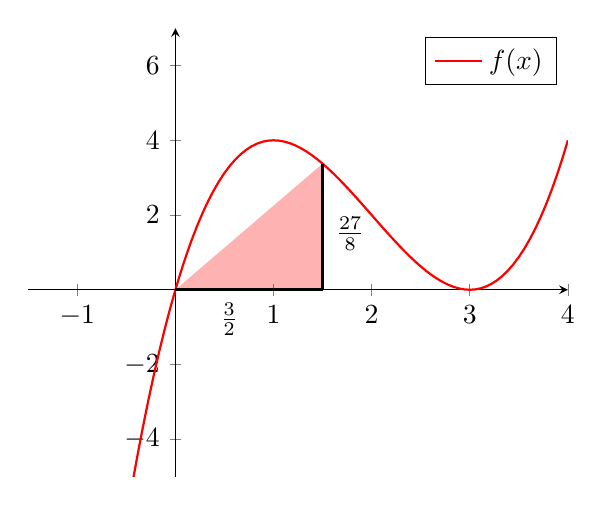
\begin{tikzpicture}   
\begin{axis}[
    axis lines=middle,
    samples=100,
    domain=-1.5:4,
    ymax=7,
    ymin=-5,
    every axis plot/.append style={thick},
]
\addplot[
    color=red,
    name path=A
]
{((\x)*(\x)*(\x))-(6*(\x)*(\x))+(9*(\x))};
\addlegendentry{$f(x)$}

\addplot[draw=none,name path=B] {((27/8)/(3/2))*(\x)};
\addplot[draw=none,name path=C] {0};
\addplot[red,opacity=0.3] fill between[of=B and C,soft clip={domain=0:1.5}];

\addplot[color=black,very thick] coordinates {(1.5,0) (1.5,3.375)};
\addplot[color=black,very thick] coordinates {(0,0) (1.5,0)};

\node[label={0:{$\frac{27}{8}$}},draw=none,inner sep=1pt] at (axis cs:1.5,1.5) {};
\node[label={250:{$\frac{3}{2}$}},draw=none,inner sep=1pt] at (axis cs:0.75,0) {};

\end{axis}
\end{tikzpicture}
\end{center}

\chapter{Integralrechnung}

\section{Stammfunktionen}

\begin{flushleft}
    Stammfunktionen sind Funktionen, die eine Funktion $f$ ergeben, wenn man sie ableitet.
    Also gilt: $F'(x)=f(x)$.

    Allgemein gilt die folgende Regel.
    \begin{align}
        f(x)&=x^n \\
        F(x)&=\frac{x^{n+1}}{n+1}+C, n \in \mathbf{R} - \{-1\}
    \end{align}
    Wenn eine Funktion abgeleitet wird fällt jede Konstante weg, daher gibt es unendlich viele Stammfunktionen, die Konstante wird mit $C$ dargestellt.
\end{flushleft}

\section{Bestimmte Integrale}

\begin{flushleft}
    Bei bestimmten Integralen ist immer klar, welches Intervall gesucht ist.
    Also gilt für ein Integral in dem Intervall $[a;b]$ diese Formel:
    \begin{align}
        \int_{a}^{b} f(x) \ dx = [F(x)]_{a}^{b}
    \end{align}
    Außerdem ist die Integralrechnung keine Flächenberechnung, daher werden oft Absolutbeträge genutzt. Damit wird das Ergebnis eines Integrals immer positiv.
    Die Definition des Absolutbetrags sieht so aus:
    \[
        \mid x \mid =
        \begin{cases}
            x, &\text{wenn } x \geq 0 \\
            -x, &\text{sonst}
        \end{cases}
    \]
\end{flushleft}

\section{Flächen zwischen zwei Funktionen}

\begin{flushleft}
    Um die Fläche zwischen den beiden Funktionen $f$ und $g$ ($f \geq g$) im Intervall $[a;b]$ zu berechnen nutzt man diese Formel:
    \begin{align}
        \int_{a}^{b} [f(x)-g(x)] \ dx
    \end{align}
\end{flushleft}

\section{Mittelwerte von Funktionen}

\begin{flushleft}
    \textbf{diskrete Mittelwerte}: \newline
    Es wird ein Mittelwert aus einer Menge von Zahlen gebildet. \newline
    \begin{align}
        \{1,3&,5,4\} \\
        \frac{1+3+5+4}{4}&=\frac{13}{4}=3.25
    \end{align}
    \newline
    \textbf{kontinuierliche Mittelwerte}: \newline
    Der Mittelwert wird aus Werten einer Funktion bestimmt. \newline
    \begin{align}
        \bar{m}=\frac{1}{b-a}\int_{a}^{b} f(x) \ dx
    \end{align}
\end{flushleft}

\section{Rekonstruktion von Beständen}

\begin{flushleft}
    Bei diesem Aufgabentyp hat man immer eine Funktion (hier: $f$) gegeben, die die momentane Änderungsrate beschreiben soll, also wie stark etwas ansteigt oder fällt. Um alle Teilaufgaben vernünftig zu lösen muss man erstmal die Stammfunktion bestimmen:
    \begin{align}
        f(x)&=F'(x) \\
        F(x)&=\int f(x) \ dx
    \end{align}
    Die Konstante $C$, die beim integrieren erscheint sollte in der Aufgabenstellung gegeben sein.
\end{flushleft}

\chapter{Weitere Regeln}

\section{Potenzgesetze}
\begin{align}
    a^0 &= 1 \\
    \frac{1}{a^n} &= a^{-n} \\
    a^n*a^m &= a^{n+m} \\
    \frac{a^n}{a^m} &= a^{n-m} \\
    a^n*b^n &= (a*b)^n \\
    \frac{a^n}{b^n} &= \left(\frac{a}{b}\right)^n \\
    \left(a^n\right)^m &= a^{n*m} \\
    a^{\frac{m}{n}} &= \sqrt[n]{a^m}=\left(\sqrt[n]{a}\right)^m
\end{align}

\section{Ableitungsregeln}
\begin{align}
    \left(x^n\right)' &=n*x^{n-1} \\
    \left(a*x^n\right)' &=a*n*x^{n-1} \\
    \left[f(x)+g(x)\right]' &=f'(x)+g'(x)
\end{align}

\section{Sigma-Umgebungen}
\begin{align}
    \sigma \approx 68.3\% \\
    2\sigma \approx 95.4\% \\
    3\sigma \approx 99.7\% \\
    1.64\sigma \approx 90\% \\
    1.96\sigma \approx 95\% \\
    2.58\sigma \approx 99\%
\end{align}

\end{document}
